\documentclass[11pt,letterpaper]{article}
\usepackage[T1]{fontenc}
\usepackage{newpxtext,newpxmath}
\usepackage[margin=0.83in,headheight=14pt,headsep=20pt,footskip=27pt]{geometry}
\usepackage{microtype,graphicx,booktabs,tabularx,array}
\usepackage[dvipsnames]{xcolor}
\usepackage{caption,subcaption,float,placeins}
\usepackage{titlesec,fancyhdr,lastpage}
\usepackage{tikz,pgfplots}
\usepackage{listings}
\usepackage{hyperref}
\usepackage{xurl}
\pgfplotsset{compat=1.18}
\usetikzlibrary{arrows.meta,positioning}
\definecolor{reportblue}{HTML}{225B70}
\definecolor{reportgray}{HTML}{555E63}
\definecolor{reportpale}{HTML}{F2F5F6}
\hypersetup{colorlinks=true,linkcolor=reportblue,citecolor=reportblue,urlcolor=reportblue,
 pdftitle={Perigee: Guided investigation of SPHEREx images},
 pdfauthor={Sathvik Loke; Sagar Raut; Akshobya Rao; Aditya Raut; Suhrit Bestavemula; Neeraj Movva},
 pdfsubject={Technical report for NASA Space Apps 2026},pdfkeywords={SPHEREx, infrared imaging, astronomy education, provenance, registration}}
\urlstyle{same}
\setlength{\parindent}{1.25em}
\setlength{\parskip}{3pt}
\linespread{1.06}
\setlength{\emergencystretch}{1.5em}
\raggedbottom
\widowpenalty=10000
\clubpenalty=10000
\titleformat{\section}{\large\bfseries}{\thesection}{0.65em}{}
\titleformat{\subsection}{\normalsize\bfseries}{\thesubsection}{0.65em}{}
\titlespacing*{\section}{0pt}{18pt}{7pt}
\titlespacing*{\subsection}{0pt}{12pt}{5pt}
\captionsetup{font=small,labelfont=bf,labelsep=period,skip=7pt}
\captionsetup[subfigure]{font=small,justification=centering}
\setlength{\textfloatsep}{17pt plus 3pt minus 2pt}
\setlength{\intextsep}{15pt plus 3pt minus 2pt}
\renewcommand{\topfraction}{0.9}
\renewcommand{\bottomfraction}{0.85}
\renewcommand{\textfraction}{0.08}
\renewcommand{\floatpagefraction}{0.8}
\renewcommand{\arraystretch}{1.25}
\newcolumntype{L}[1]{>{\raggedright\arraybackslash}p{#1}}
\pagestyle{fancy}
\fancyhf{}
\fancyhead[L]{\small\textsc{Perigee}\quad\textcolor{reportgray}{Technical report}}
\fancyhead[R]{\small\textcolor{reportgray}{15 November 2026}}
\fancyfoot[L]{\footnotesize\textcolor{reportgray}{NASA Space Apps 2026}}
\fancyfoot[R]{\footnotesize\thepage\ /\ \pageref*{LastPage}}
\renewcommand{\headrulewidth}{0.3pt}
\renewcommand{\footrulewidth}{0pt}
\lstset{basicstyle=\ttfamily\footnotesize,backgroundcolor=\color{reportpale},
 breaklines=true,columns=fullflexible,keepspaces=true,frame=single,
 rulecolor=\color{reportpale},framesep=7pt,xleftmargin=8pt,xrightmargin=8pt}
\newcommand{\micron}{\ensuremath{\mu\mathrm{m}}}
\newcommand{\arcsec}{\ensuremath{^{\prime\prime}}}
\newcommand{\repo}[2]{\href{https://github.com/sathvikloke/perigee/#1}{#2}}
\newcommand{\observation}[3]{\begin{subfigure}[t]{#1\linewidth}\centering
 \colorbox{black}{\includegraphics[width=\dimexpr\linewidth-2\fboxsep\relax]{#2}}\caption{#3}\end{subfigure}}
\begin{document}
\thispagestyle{plain}
\begin{center}
 {\small\scshape Technical report\quad |\quad NASA Space Apps 2026}\par
 \vspace{12pt}
 {\LARGE\bfseries Perigee: Guided investigation\\[4pt]of SPHEREx images}\par
 \vspace{13pt}
 {Sathvik Loke\quad Sagar Raut\quad Akshobya Rao}\\[4pt]
 {Aditya Raut\quad Suhrit Bestavemula\quad Neeraj Movva}\par
 \vspace{8pt}
 {\small Team Perigee, Planet X and SPHEREx challenge}\par
 {\small 15 November 2026}
\end{center}
\vspace{6pt}
\begin{abstract}
Perigee is a browser application for comparing NASA SPHEREx infrared observations and recording what those comparisons support. Students can start with a guided investigation, inspect observation dates and wavelengths, check pixel quality, and export an explanation with its source records. We built three investigations around apparent motion in Barnard's Star, time and wavelength comparisons of Epsilon Indi B, and a flagged feature in the WISE 0855 field. The processing pipeline converts archive FITS cutouts into images on a fixed sky grid and retains the metadata needed to reproduce the view. Our retained dataset contains 183 unique cutouts from five fields. An independent field-star registration check returned 128 PASS and 55 UNKNOWN verdicts, with no FAIL verdicts; tests with deliberately displaced pixels rejected all tested shifts of 1, 2 and 5 native pixels on three selected frames. The report describes the implementation, case evidence and checks behind these results. Perigee's contribution is a guided comparison workflow in which a learner's explanation remains connected to the observations and processing choices used to reach it.
\end{abstract}
\vspace{4pt}
\noindent\textbf{Keywords:} SPHEREx; infrared imaging; astronomy education; image registration; data provenance.

\section{Purpose and contribution}
A bright feature shifts between two astronomical images. A learner can see the difference before knowing whether it comes from motion, a different wavelength, display contrast or an unreliable pixel. Interpreting the image requires the observation context as well as the image itself. Perigee puts those checks beside a comparison and asks the learner to explain the result.

We built the application for students, teachers and astronomy clubs. A student can work through a case and save an evidence card; a teacher can use that card to examine both the reasoning and the source observations. A club can use the cases for a demonstration, then search another object or sky position. These are intended uses. We report implementation and scientific checks here; educational benefit remains a question for a classroom evaluation.

The project combines archive access, guided cases and editable evidence records in one workflow. Existing tools already provide archive search, image playback and quality information. Our review of SPHEREx Explorer found overlap in those functions and in authored investigations. The contribution we pursue is the connection between a learner's written explanation and the exact observations, display settings and quality checks used in the comparison~\cite{comparison}. The review included static code and API inspection where interactive access was limited.

\section{Application and investigation workflow}
The public application opens without an account. A learner chooses a case, reads the instruction above the images, and plays a comparison. The interface labels date and wavelength differences, provides a catalog-position marker, and offers an overlay for flagged pixels. Figure~\ref{fig:app} shows the Barnard's Star comparison.

The notebook begins with an observation, then asks for an explanation and remaining uncertainty. A learner can compare the completed response with the case reference and revise the notes. The evidence card stores the selected frame identifiers, observation times, target wavelengths, quality summaries, display settings and source links alongside the response. The browser saves the latest notes locally; exports are available as JSON and printable PDF~\cite{notebook}. A teacher can read an exported card without having to reconstruct which images a student selected.

\begin{figure}[htbp]
 \centering
 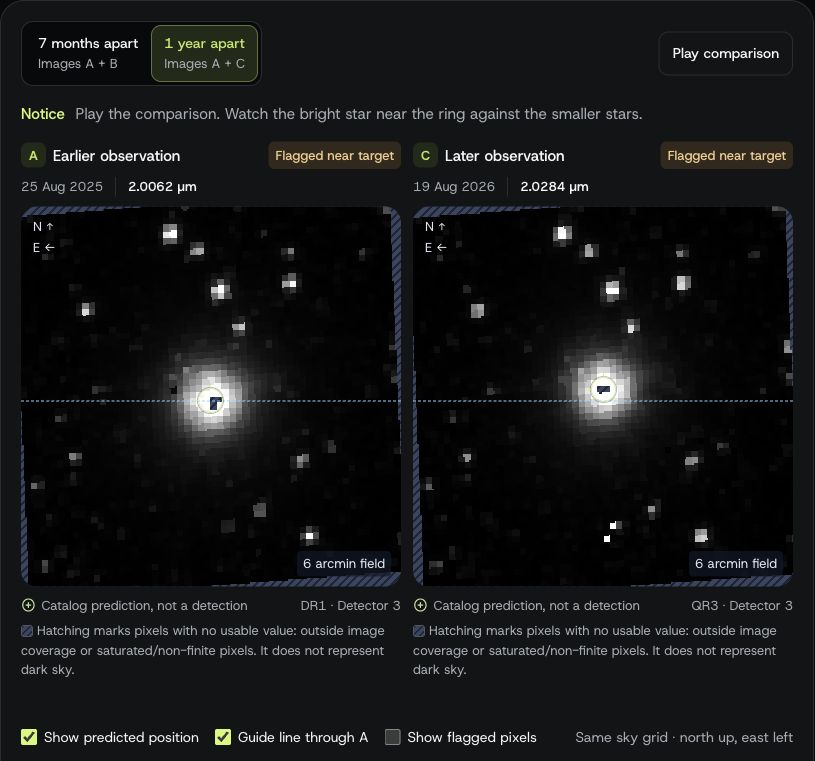
\includegraphics[width=0.73\linewidth]{../presentation/standalone-assets/barnard-app.png}
 \caption{The current Barnard's Star comparison in Perigee. The selected pair places observations from August 2025 and August 2026 on the same sky grid. The instruction, playback controls, dates and wavelengths sit above the images. The image markers show catalog predictions; they do not mark a fitted detection. This is a capture of the running application.}
 \label{fig:app}
\end{figure}

Curated cases use processed archive observations bundled with the release. General exploration accepts object names through the Sesame resolver or sky coordinates, searches the archive and requests frames as they become available. The React/TypeScript client runs on Cloudflare; a Python/FastAPI service handles live archive access and processing. The client limits frame requests to two at a time, retries transient failures with bounded backoff, and caches completed frames. A failed request retains its place in the results and offers a retry. Live requests still depend on IRSA response time: release probes on 15 November included a search that exceeded the API's timeout~\cite{release}. The bundled cases provide the same comparison and notebook workflow without a new FITS download for each session.

Saved notes, the other investigations and five named target fields give a learner a reason to return. The current notebook holds the latest local response, so sharing with a teacher requires exporting it or using the same device. The implementation does not provide a class roster or a full history of revisions.

\FloatBarrier
\section{Data sources and image processing}
\subsection{Archive inputs and provenance}
We use SPHEREx Level 2 spectral images from NASA/IPAC's Infrared Science Archive (IRSA), drawing from Data Release 1 (DR1) and Quick Release 3 (QR3). IRSA provides a Simple Image Access service for locating observations and a cutout service for requesting a small field from an image~\cite{irsa,access}. Our retained set covers Barnard's Star, Epsilon Indi B, WISE 0855, RW Aurigae and R Draconis. The 183 unique cutouts represent 109 exposures; simultaneous observations on different detectors remain distinct cutouts.

For each frame, we retain the observation identifier, detector, collection, original archive URL, cutout URL, retrieval time and SHA-256 hash of the retained bytes. The case definitions identify the selected records and their roles~\cite{cases}. Raw FITS files remain outside Git, while processed previews and metadata are committed. A reviewer can follow an image back to the archive and check the retained file's identity without relying on its appearance.

SIMBAD supplies target positions and proper motions~\cite{simbad}. We propagate the catalog position to the observation epoch for the displayed marker. Annual parallax is omitted from this propagation. Gaia DR3 supplies a separate set of field stars for the registration audit~\cite{gaia,registration}. The target prediction and the field-star check answer different questions: one locates the expected target, and the other tests the image coordinates against surrounding stars.

\begin{figure}[htbp]
 \centering
 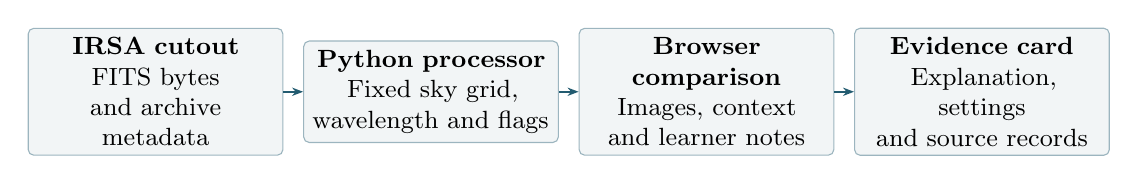
\begin{tikzpicture}[node distance=0.25cm, every node/.style={font=\small},
 stage/.style={draw=reportblue!45,fill=reportpale,rounded corners=2pt,
 text width=3.0cm,minimum height=1.25cm,align=center},
 flow/.style={-{Stealth[length=4pt]},draw=reportblue,line width=0.6pt}]
 \node[stage] (a) {\textbf{IRSA cutout}\\FITS bytes\\and archive metadata};
 \node[stage,right=of a] (b) {\textbf{Python processor}\\Fixed sky grid,\\wavelength and flags};
 \node[stage,right=of b] (c) {\textbf{Browser comparison}\\Images, context\\and learner notes};
 \node[stage,right=of c] (d) {\textbf{Evidence card}\\Explanation, settings\\and source records};
 \draw[flow] (a)--(b);\draw[flow] (b)--(c);\draw[flow] (c)--(d);
 \end{tikzpicture}
 \caption{Processing and evidence flow. The processor receives bytes and metadata; archive requests take place outside it. Source identifiers and processing settings accompany the preview into the exported evidence card.}
 \label{fig:pipeline}
\end{figure}

\subsection{A fixed sky grid}
The processor reads the \texttt{IMAGE}, \texttt{VARIANCE} and \texttt{FLAGS} extensions of each Flexible Image Transport System (FITS) file. It uses the mid-exposure \texttt{DATE-AVG} and \texttt{MJD-AVG} values, checks file identity and detects truncated data units. Before WCSLIB evaluates a spectral lookup, the processor checks that its index is finite and strictly monotonic~\cite{processor}.

We sample each image onto a tangent-plane grid centered on the query, with north up and east left. The default view spans 6 arcminutes across 256 pixels:
\begin{equation}
 s=\frac{6\times60}{256}=1.40625\ \text{arcsec per display pixel}.
 \label{eq:scale}
\end{equation}
Nearest-neighbor sampling retains the discrete native pixel structure. The output grid stays fixed as the target moves. Display pixels are smaller than the native detector sampling and do not add angular resolution.

The processor evaluates wavelength and bandwidth at the predicted native target position using the alternate spectral world coordinate system (WCS) and the \texttt{WCS-WAVE} table. It removes celestial SIP distortion for that spectral lookup and returns no wavelength for an off-image position. The resulting values describe the band sampled at the marker; the preview does not constitute a calibrated spectrum.

\subsection{Contrast and pixel quality}
For a finite image value $I$, display limits $L$ and $H$, and softening parameter $a=10$, the normalized stretch is
\begin{equation}
 t=\operatorname{clip}\!\left(\frac{I-L}{H-L},0,1\right),\qquad
 g=255\,\frac{\operatorname{asinh}(a\,t)}{\operatorname{asinh}(a)}.
 \label{eq:stretch}
\end{equation}
The processor rounds $g$ to an 8-bit gray value. Unless a case supplies shared limits, $L$ and $H$ are the 1st and 99.5th percentiles of finite grid values. Shared limits assign the same gray value to the same input value across a pair. Separate limits can make equal values look different. The interface therefore identifies the display scale used for each comparison.

Pixel flags accompany the images. The target quality screen examines a circle of radius 2.5 native pixels around the predicted position, while the overlay allows inspection elsewhere in the frame. \texttt{SOURCE} and \texttt{FULLSAMPLE} are informational bits and are separate from problem flags. A clear target screen means no screened problem at that location; it does not establish a source detection or certify the rest of the image. The preview pipeline performs neither background subtraction nor photometric measurement.

\section{Three guided investigations}
\subsection{Barnard's Star: apparent motion}
The Barnard case uses D3 observations from 25 August 2025, 19 March 2026 and 19 August 2026, at target wavelengths of 2.0062, 2.0123 and 2.0284\,\micron. The first and last images span about a year, use a shared display scale and sample similar wavelengths (Figure~\ref{fig:barnard}). The learner watches the bright source relative to the surrounding stars, then checks whether the dates and image quality support a movement claim.

\begin{figure}[htbp]
 \centering
 \observation{.34}{../../backend/content/presets/barnards_star/case-moving_neighbor/2025W35_1A_0008_1_D3.png}{25 Aug 2025; 2.0062\,\micron}\hspace{0.06\linewidth}
 \observation{.34}{../../backend/content/presets/barnards_star/case-moving_neighbor/2026W34_1A_0431_1_D3.png}{19 Aug 2026; 2.0284\,\micron}
 \caption{Barnard's Star, full 6-arcminute fields on the same sky grid, with north up and east left. These are the original processed case PNGs, with shared contrast limits and no added image features. The bright central glow shifts north. Its saturated core limits the comparison to qualitative motion. Data: NASA/IPAC IRSA, SPHEREx DR1 and QR3.}
 \label{fig:barnard}
\end{figure}

The catalog prediction shifts by 7.29 display pixels between the first and last frames, or about 10.25\arcsec. Eleven variations of a glow-position proxy produce northward shifts of 6.87 to 8.87 display pixels; selected field stars move at most 0.83 display pixels~\cite{controls}. The agreement in direction supports the visible relative shift. Saturation and non-finite pixels make the inferred center depend on the window and weighting. We therefore use the glow as a visual consistency check and retain the spread across methods, rather than deriving a precise proper motion. All 34 retained Barnard cutouts pass the separate field-star registration check~\cite{registration}.

\FloatBarrier
\subsection{Epsilon Indi B: separating time from wavelength}
The Epsilon case gives the learner two different comparisons (Figure~\ref{fig:epsilon}). A and B are observations from 29 April and 27 September 2026 at 2.3232 and 2.3220\,\micron. A and C share the April exposure, but C samples 4.9399\,\micron\ on detector D6. A difference between A and C cannot establish change over time because both observations occurred at the same instant. Detector response and display scale also affect their appearance.

\begin{figure}[htbp]
 \centering
 \observation{.31}{../../backend/content/presets/epsilon_indi_b/case-fair_comparison/2026W18_1A_0516_1_D3.png}{A: 29 Apr 2026; 2.3232\,\micron}\hfill\observation{.31}{../../backend/content/presets/epsilon_indi_b/case-fair_comparison/2026W39_2A_0597_4_D3.png}{B: 27 Sep 2026; 2.3220\,\micron}\hfill\observation{.31}{../../backend/content/presets/epsilon_indi_b/case-fair_comparison/2026W18_1A_0516_1_D6.png}{C: 29 Apr 2026; 4.9399\,\micron}

 \caption{The Epsilon Indi B case. A--B compares dates at similar wavelengths; A--C compares wavelengths at the same time. Each panel shows the full 6-arcminute field. A and B use their case's shared display limits; C uses a separate stretch. Gray levels across A and C therefore cannot supply a brightness ratio. Original processed PNGs from NASA/IPAC IRSA observations.}
 \label{fig:epsilon}
\end{figure}

C has too few supporting field stars for the independent registration test and retains an UNKNOWN verdict. A same-exposure control places its target within 0.15\arcsec\ of the position in Gaia-checked frame A~\cite{registration}. This constrains the relative position at the target, assuming A is correct, but supplies no independent test of rotation or scale across C. The learner's task is to identify what the chosen pair compares and state an explanation consistent with that context.

\subsection{WISE 0855 field: a flagged feature}
The third case uses SPHEREx observations of the field around WISE 0855. The first pair dates from 7 and 10 November 2025 at nearly the same target wavelength, about 1.2572\,\micron. A third observation from 11 May 2026 samples about 1.4443\,\micron. One bright feature appears to jump in the first pair while nearby stars remain aligned (Figure~\ref{fig:wise}). The feature is not identified as WISE 0855.

The feature occupies the same detector pixel, $(1709,1364)$, in both early observations, yet lands 5.36\arcsec\ apart on the common sky grid. Three usable field stars agree within 0.76\arcsec. Their detector displacement predicts a 5.38\arcsec\ displacement for a detector-fixed pixel~\cite{controls}. Both observations flag the feature with \texttt{TRANSIENT}, \texttt{SUR\_ERROR} and \texttt{NONFUNC}; the additional \texttt{SOURCE} bit in the first frame is informational. The detector coordinates and flags support treating the apparent jump as unreliable evidence for a moving celestial source. They do not establish the physical cause of the detector feature.

\begin{figure}[htbp]
 \centering
 \begin{subfigure}{.31\linewidth}\centering
 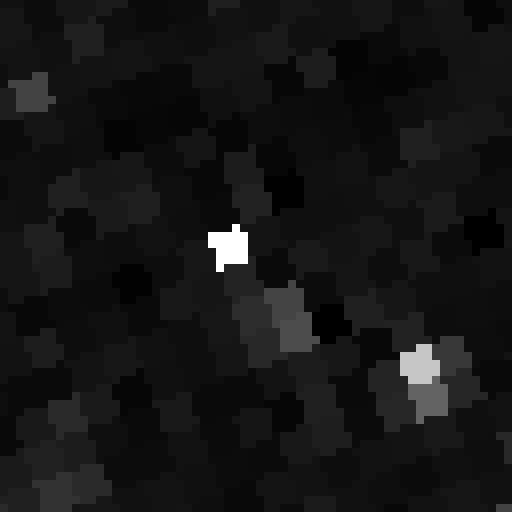
\includegraphics[width=\linewidth]{generated/wise-A-sky.png}
 \caption{7 Nov 2025}\end{subfigure}\hspace{.04\linewidth}
 \begin{subfigure}{.31\linewidth}\centering
 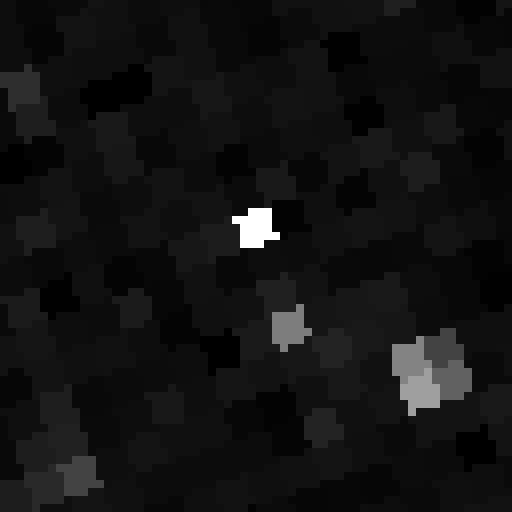
\includegraphics[width=\linewidth]{generated/wise-B-sky.png}
 \caption{10 Nov 2025}\end{subfigure}\\[7pt]
 \begin{subfigure}{.31\linewidth}\centering
 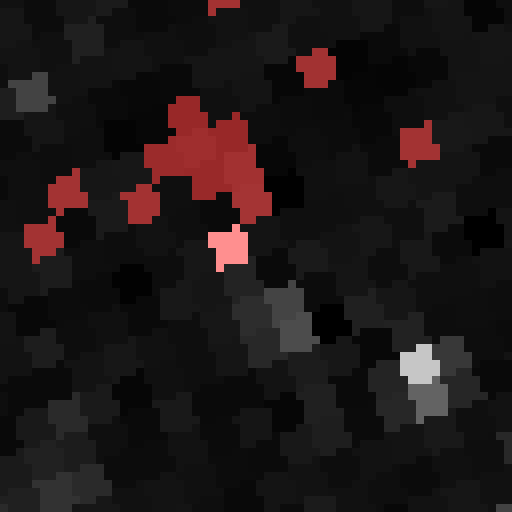
\includegraphics[width=\linewidth]{generated/wise-A-flags.png}
 \caption{Same crop, problem flags}\end{subfigure}\hspace{.04\linewidth}
 \begin{subfigure}{.31\linewidth}\centering
 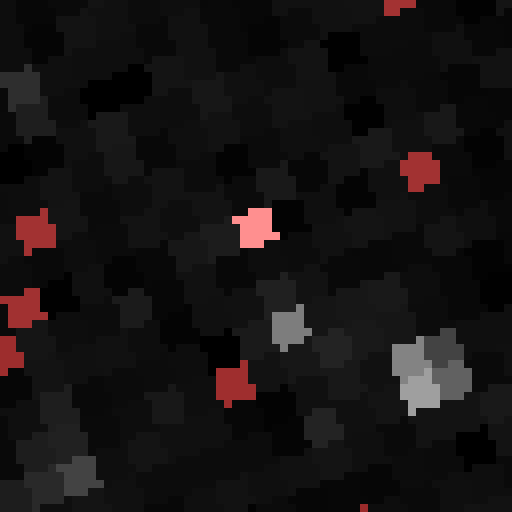
\includegraphics[width=\linewidth]{generated/wise-B-flags.png}
 \caption{Same crop, problem flags}\end{subfigure}
 \caption{The jumping feature in the WISE 0855 field. Each panel crops the same 90-arcsecond square from the fixed sky grid, with north up and east left. The bright feature near the center shifts relative to the neighboring star below and to its right. Red marks are the existing problem-flag overlay. Both dates place the feature at detector pixel $(1709,1364)$. The panels preserve the source pixel values and per-frame contrast; nearest-neighbor enlargement adds no image detail. Data: NASA/IPAC IRSA; feature identification from the retained controls~\cite{controls}.}
 \label{fig:wise}
\end{figure}

\FloatBarrier
\section{Validation and controlled comparisons}
\subsection{Internal consistency and independent registration}
The historical acceptance sweep contains 189 product records: 183 unique cutouts and six case copies with different rendering settings. All 189 records passed the original seven checks for consistency with FITS bytes, metadata and rendering rules~\cite{acceptance}. Those checks reproduce timestamps, wavelength lookup, masks, geometric coverage, stretch and file hashes. Four records were geometrically outside coverage. Saturation at a covered position remains a quality condition, distinct from missing coverage.

A reconstruction that uses the image's own WCS header can reproduce an erroneous alignment. We therefore implemented a separate registration check using Gaia field stars. It starts with detections selected without a catalog or WCS, votes for a common offset from Gaia positions, and tests rotation~\cite{registration}. This prevents a large offset from removing all candidate associations and leaving a frame with an unsupported pass.

The audit returned 128 PASS, 55 UNKNOWN and 0 FAIL verdicts on 183 unique cutouts (Figure~\ref{fig:registration}). Including repeated case records gives 133 PASS and 56 UNKNOWN. We keep these denominators separate. UNKNOWN means insufficient support for a verdict; it contributes no pass to the total.

\begin{figure}[htbp]
 \centering
 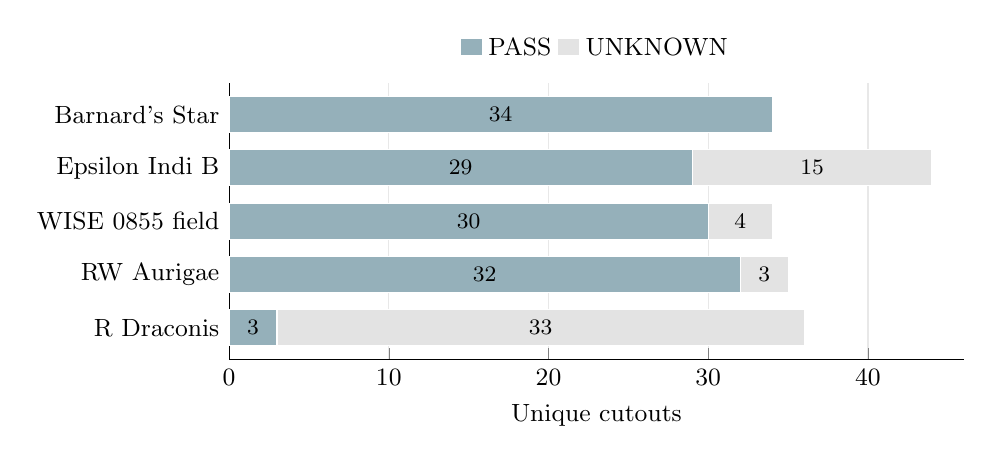
\begin{tikzpicture}
\begin{axis}[xbar stacked,width=.90\linewidth,height=5.1cm,
 xmin=0,xmax=46,ymin=-.6,ymax=4.6,bar width=13pt,
 ytick={0,1,2,3,4},yticklabels={R Draconis,RW Aurigae,WISE 0855 field,Epsilon Indi B,Barnard's Star},
 axis lines*=left,xlabel={Unique cutouts},xtick={0,10,20,30,40},
 tick label style={font=\small},label style={font=\small},
 xmajorgrids=true,grid style={gray!18},
 legend style={draw=none,font=\small,at={(.5,1.04)},anchor=south,legend columns=2},
 nodes near coords,point meta=explicit symbolic,nodes near coords style={font=\footnotesize,color=black}]
\addplot[fill=reportblue!48,draw=white] coordinates {(34,4)[34] (29,3)[29] (30,2)[30] (32,1)[32] (3,0)[3]};
\addplot[fill=gray!22,draw=white] coordinates {(0,4)[] (15,3)[15] (4,2)[4] (3,1)[3] (33,0)[33]};
\legend{PASS,UNKNOWN}
\end{axis}\end{tikzpicture}

 \caption{Independent registration verdicts by target field, derived from the committed per-frame audit. The bars count unique cutouts and sum to 183. PASS requires enough supporting stars under the stated thresholds; UNKNOWN retains frames without adequate support. No retained cutout received FAIL. The selected fields do not supply an all-sky reliability estimate.}
 \label{fig:registration}
\end{figure}

The check reports FAIL for an offset above 0.6 native pixels at more than four standard errors. It also tests for rotation, using the support and significance rules in the audit implementation. Fewer than three detections or supporting pairs produces UNKNOWN. We set the thresholds after examining the retained frames and before testing injected perturbations, so these results describe the selected set rather than a held-out generalization test.

\subsection{Injected shifts and sensitivity}
On three selected real frames, deliberate shifts of 1, 2 and 5 native pixels all produced FAIL, with recovered offsets within 0.2 native pixels of the injected values. The older header-based check passed some 2- and 5-pixel shifts after losing the Gaia associations. The independent check catches that failure mode. Table~\ref{tab:controls} records the tested sensitivity, including the conditions under which evidence remains insufficient.

\begin{table}[htbp]
 \caption{Registration perturbation checks. Native pixels and display pixels are different units; the default display scale is given in Equation~\ref{eq:scale}. Full fixture results and thresholds are in the registration audit~\cite{registration}.}
 \label{tab:controls}
 \small\centering
 \begin{tabularx}{\linewidth}{@{}L{.27\linewidth}X@{}}
 \toprule
 \textbf{Perturbation or condition}&\textbf{Retained result}\\\midrule
 1, 2 and 5 native-pixel shifts & FAIL for all nine tested frame--shift combinations across three real frames.\\
 Shifts of 0.5 native pixels or less & Not reliably rejected by either validator.\\
 Rotation near $1^\circ$ & Detected in sufficiently rich fields; sparse fields can retain PASS.\\
 Rotation of $3^\circ$ & FAIL or UNKNOWN on the tested sparse fixtures, depending on remaining support.\\
 Fewer than three supporting detections & UNKNOWN, including the Epsilon D6 case.\\\bottomrule
 \end{tabularx}
\end{table}

An earlier selected-match analysis retained 958 stars in 156 unique frames. The median of the per-frame median PNG residuals was 0.45 display pixels. Its filters required a peak signal-to-noise ratio of at least 15, association within one native pixel of Gaia, and suitable measurement windows. The retained sample includes 189 catalog-ambiguous stars. That statistic describes those selected matches and is separate from the stricter 128-PASS result. We use the independent verdicts when stating coverage of the registration check.

\subsection{Controls for interpreting visual change}
The deterministic controls test the explanations used in the cases~\cite{controls}. A display experiment maps the same input value, 1.0\,MJy\,sr$^{-1}$, to gray levels 156 and 174 under two per-frame stretches. Shared limits map it to 159 in both. This demonstrates a display-induced difference without changing the underlying value. The physical background in the second WISE-field image was about 0.971 times the first; shared stretching leaves that difference intact, and its cause remains undetermined.

The time-and-wavelength check places the first WISE-field pair 2.655 days apart and only 0.0018 bandwidths apart at the target. The Epsilon A--C pair instead shares an exposure and spans 69.6 bandwidths across different detectors. These controls establish why a date comparison and a wavelength comparison require different explanations. An information-removal matrix records which of 16 questions can be addressed by 11 representations of the same observations. It tests what information each representation supplies, rather than how learners perform on it.

\section{Use and interpretation}
Perigee provides a complete short task: inspect a comparison, check the observation context and save a reasoned response. A finished Barnard card can state that the bright source shifts north relative to surrounding stars, cite the dates and similar wavelengths, and explain that saturation prevents a precise position measurement. The source records allow a reader to inspect those choices. The result is more useful for discussing evidence than an image alone because the explanation and its basis remain together.

The scientific output consists of teaching comparisons, processing records and validation results. The display supports qualitative inspection; quantitative fluxes, variability amplitudes and proper motions require additional measurement procedures. Marker uncertainty includes the input catalog astrometry and omitted annual parallax. For Barnard's Star, the reported parallax amplitude is about 0.547\arcsec, or 0.39 display pixels, which matters if someone tries to interpret the marker as an exact apparent position~\cite{registration}.

The educational contribution can be evaluated by asking learners to interpret an unfamiliar comparison before and after using a case. A predefined rubric could score whether their explanations account for dates, wavelength, display scale and quality. That study remains proposed. The present report establishes the implemented workflow and the retained evidence behind its examples.

\FloatBarrier
\section{Reproducibility and artifact access}
The repository contains the processor, case definitions, processed previews, cached Gaia control catalogs and review outputs. Table~\ref{tab:source} identifies the entry points. The public app and source are available at \url{https://perigee.lokesathvik.workers.dev/} and \url{https://github.com/sathvikloke/perigee}.

\begin{table}[htbp]
 \caption{Source locations for the methods and evidence in this report. Paths are relative to the public repository.}
 \label{tab:source}
 \small\centering
 \begin{tabularx}{\linewidth}{@{}L{.51\linewidth}X@{}}
 \toprule\textbf{Repository path}&\textbf{Contents}\\\midrule
 \path{backend/data/process.py}&FITS parsing, fixed grid, spectral lookup, masks, stretch and provenance.\\
 \path{backend/data/archive.py}&Archive search and cutout requests.\\
 \path{backend/content/cases/}&Case text, selected observations and source identifiers.\\
 \path{science/reviews/acceptance/}&Consistency checks and corrected astrometry column.\\
 \path{science/reviews/registration-audit/}&Independent verdicts, perturbation fixtures and residuals.\\
 \path{science/reviews/overnight-controls/}&Display, quality and comparison controls.\\
 \path{frontend/src/components/Notebook.tsx}&Learner response, local save and evidence export.\\\bottomrule
 \end{tabularx}
\end{table}

To rerun the scientific checks, install the repository's Python requirements and Pillow, then set \texttt{DATA} to the retained raw FITS directory. That directory must contain the manifest and cutouts named by the scripts. Use new output directories: the audit refuses to overwrite a non-empty destination.

\begin{lstlisting}
python science/reviews/acceptance/check_acceptance.py \
  --data-root "$DATA" --all --out /tmp/acceptance-review.json

python science/reviews/registration-audit/audit_registration.py \
  --data-root "$DATA" --out-dir /tmp/registration-review

python science/reviews/overnight-controls/run_controls.py \
  --data-root "$DATA" --out /tmp/controls-review

PERIGEE_BUILD_DATA="$DATA" python -m pytest \
  science/reviews/registration-audit/tests -q -p no:cacheprovider
\end{lstlisting}

The retained control environment records Python 3.12.16, NumPy 2.5.4, Astropy 8.0.2 and Pillow 13.0.0. Two control runs matched numerically; manifest timestamps, runtime and output paths differed. OS fonts can change figure pixels. This report assembles the committed experiment results and does not claim a new experiment run.

To check provenance without the raw dataset, open a case definition and its frame records, then follow the archive links and compare observation identifiers, release, detector and hash fields. Matching a stored cutout hash requires the same bytes; a different archive build or cutout request may produce a different file. The report source and figure-generation script live in \path{docs/report/}. Tectonic compiles the LaTeX document, embeds the fonts and preserves selectable text.

\section*{Acknowledgments}
We use SPHEREx data from NASA/IPAC IRSA. SPHEREx is a joint project of the Jet Propulsion Laboratory and the California Institute of Technology, funded by NASA. IRSA operates at Caltech under contract with NASA. We acknowledge CDS for SIMBAD and ESA and the Gaia collaboration for Gaia DR3. The image panels contain processed archive observations; the interface figure is an application screenshot. Development and writing assistance are documented in the repository's \href{https://github.com/sathvikloke/perigee/blob/main/docs/AI_USE.md}{AI-use notes}.

\begin{thebibliography}{99}
\small
\setlength{\itemsep}{5pt}
\bibitem{challenge} NASA Space Apps. \emph{Planet X and SPHEREx}, 2026 challenge. \url{https://www.spaceappschallenge.org/2026/challenges/planet-x-and-spherex/}.
\bibitem{irsa} NASA/IPAC IRSA. \emph{SPHEREx Data Release 1 overview}. DR1 spectral images: \href{https://doi.org/10.26131/IRSA678}{doi:10.26131/IRSA678}. \url{https://irsa.ipac.caltech.edu/data/SPHEREx/docs/overview_dr1.html}.
\bibitem{access} Caltech/IPAC. \emph{SPHEREx data access}. Archive user guide, 12 November 2026. \url{https://caltech-ipac.github.io/spherex-archive-documentation/spherex-data-access/}.
\bibitem{simbad} Centre de Donn\'ees astronomiques de Strasbourg. \emph{SIMBAD astronomical database}. \url{https://simbad.cds.unistra.fr/}.
\bibitem{gaia} ESA and the Gaia collaboration. \emph{Gaia Data Release 3}. \url{https://www.cosmos.esa.int/web/gaia/dr3}.
\bibitem{comparison} Team Perigee. \emph{Contribution and closest-work review}, 2026. \repo{blob/main/science/reviews/contribution/README.md}{Repository review and source comparisons}.
\bibitem{cases} Team Perigee. \emph{Guided case definitions}: moving neighbor, fair comparison and WISE 0855 quality case, 2026. \repo{tree/main/backend/content/cases}{Case records, archive links and hashes}.
\bibitem{processor} Team Perigee. \emph{SPHEREx image processor}, version \texttt{perigee-processor-a/0.1.2}. \repo{blob/main/backend/data/process.py}{Processing source}; \repo{blob/main/backend/data/archive.py}{archive client}.
\bibitem{acceptance} Team Perigee. \emph{Acceptance checks and corrected registration scope}, 14--15 November 2026. \repo{tree/main/science/reviews/acceptance}{Scripts, cached catalogs and results}.
\bibitem{registration} Team Perigee. \emph{Registration and astrometric-validity audit}, 14--15 November 2026. \repo{tree/main/science/reviews/registration-audit}{Methods, per-frame verdicts, perturbation controls and tests}.
\bibitem{controls} Team Perigee. \emph{Deterministic comparison controls}, 15 November 2026. \repo{tree/main/science/reviews/overnight-controls}{Code, manifests, numerical results and figures}.
\bibitem{notebook} Team Perigee. \emph{Investigation notebook and evidence export}, 2026. \repo{blob/main/frontend/src/components/Notebook.tsx}{Notebook source}; \repo{tree/main/docs/presentation/rehearsal}{retained evidence-card examples}.
\bibitem{release} Team Perigee. \emph{Release observations}, 15 November 2026. \repo{blob/main/qa/landing-motion/RELEASE.md}{Public smoke probes and direct-archive timing}.
\end{thebibliography}
\end{document}
